% !TeX root = ba.tex

\section{Experiments}
\label{sec:experiments}

\subsection{Datasets and Network Architectures}

We trained models on each of the following benchmark data sets:

\begin{itemize}
	\item MNIST: $28\times28$ grayscale images of handwritten digits ($60000$  images for training, $10000$  images for testing) \cite{mnist}
	\item Fashion-MNIST:  $28\times28$ grayscale images of fashion items ($60000$ images for training, images $10000$ for testing) \cite{fashion}
	\item SVHN: $32\times32$ color images of house numbers ($73257$  images for training, $26032$ images for testing) \cite{svhn}
	\item CIFAR-10: $32\times32$ color images of animals and vehicles ($50000$  images for training, $10000$  images for testing) \cite{cifar}
\end{itemize}

Each of the four data sets consists of ten classes.

As baseline architectures we trained convolutional networks utilizing max pooling, batch normalization \citep{batchnorm} and dropout \citep{dropout}.
Training capsule networks can be comparatively more difficult in practice, therefore we had to carefully construct well-suited architectures:

For the MNIST data set we used a three layer CapsNet like that of \citet{capsules}, but with only 64 convolutional kernels in the first layer.
For the Fashion-MNIST and the SVHN data sets we used CapsNets with two convolutional layers in the beginning, followed by the primary capsule layer and the class capsules.

Simple CapsNets however do not perform very well on more complex data like \mbox{CIFAR-10} \citep{complex}, therefore we use a modified DCNet \citep{dcnet} with three convolutional capsule layers and a non-of-the-above category (see \Cref{sec:capsules}) for the dynamic routing.

We train all CapsNets using margin loss and the reconstruction loss for regularization \citep{capsules}, and we use three iterations in the routing algorithm.
All CapsNets as well as ConvNets are trained with the Adam optimizer \citep{adam}.
For more details on the model architectures, please refer to the tables in \Cref{lab:networks}.

The test accuracies of our networks on the respective data sets are displayed in \Cref{tab:accuracies}.
While these accuracies do not reach the state of the art, the similarity between the performances of the CapsNets and ConvNets indicates their suitability for the task of comparing adversarial robustness.

\begin{table}	
	\centering
	\begin{tabular}{lcccc}
		\toprule
		Network       & MNIST & Fashion-MNIST & SVHN & CIFAR-10  \\
		\midrule
		ConvNet           & $99.39\%$ & $92.90\%$ & $92.57\%$ & $88.22\%$ \\
		CapsNet           & $99.40\%$ & $92.65\%$ & $92.35\%$ & $88.21\%$ \\
		\bottomrule\\
	\end{tabular}
	\caption[Test accuracies]{Test accuracies achieved by our networks}
	\label{tab:accuracies}
\end{table}

For each of the data sets we compute adversarial examples using our four chosen attacks in the following manner:\\
We randomly select $1000$ images each from the test set and attack them with DeepFool and the Boundary attack.
For Carlini-Wagner (with hyperparameter $\kappa=1$) we calculate $500$ adversarial examples for randomly chosen images from the test set and randomly chosen target labels (that are different from the true labels).
We make five steps with the binary search for the $c$ value in \Cref{eq:cwproblem}, but we determine a favorable initial value for $c$ by performing some runs with more iterations for each architecture and dataset combination.
In the case of the universal perturbation we divide the test set into ten parts and compute on each part ten adversarial perturbations.

We do not restrict the maximal perturbation norm for any of the attacks and hence the Carlini-Wagner, the boundary and the DeepFool attack only generate valid adversarial examples.
Regarding the universal perturbations, we terminate the algorithm once accuracy falls below $50\%$.
We found that the universal perturbations generalize well: while only a tenth of the test set is used to generate each universal perturbation, they can reduce the accuracy on the whole test set to $50\pm2.5\%$.

In \Cref{fig:images} some examples of the product of the attacks on CIFAR-10 can be seen.
The Carlini-Wagner, the boundary and the DeepFool attack result in humanly imperceptible adversarial examples.
Only the universal perturbations are clearly visible.
Furthermore we can observe some differences in the structure of the adversarial perturbations.
While the black-box attack (Boundary attack) produces perturbations that resemble random noise, some noticeable patterns emerge in the perturbations of the white-box attacks.
For more examples of adversarial images for this and the other datasets, see \Cref{lab:images}.

\begin{center}
\begin{longtable*}{m{1.6cm}m{2.2cm}m{4.2cm}m{4.2cm}}
	\raggedleft CW & 
	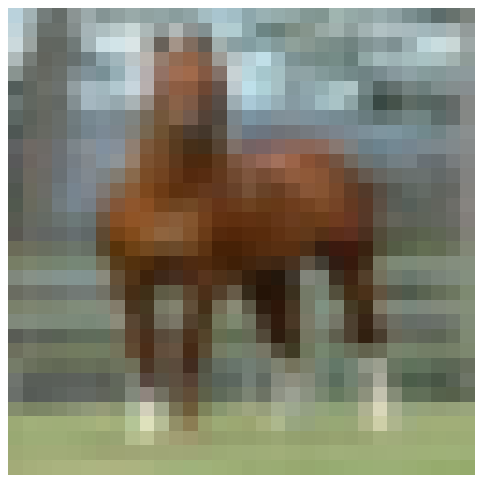
\includegraphics[height=2cm]{cifar10_carlini_wagner_orig.pdf} & 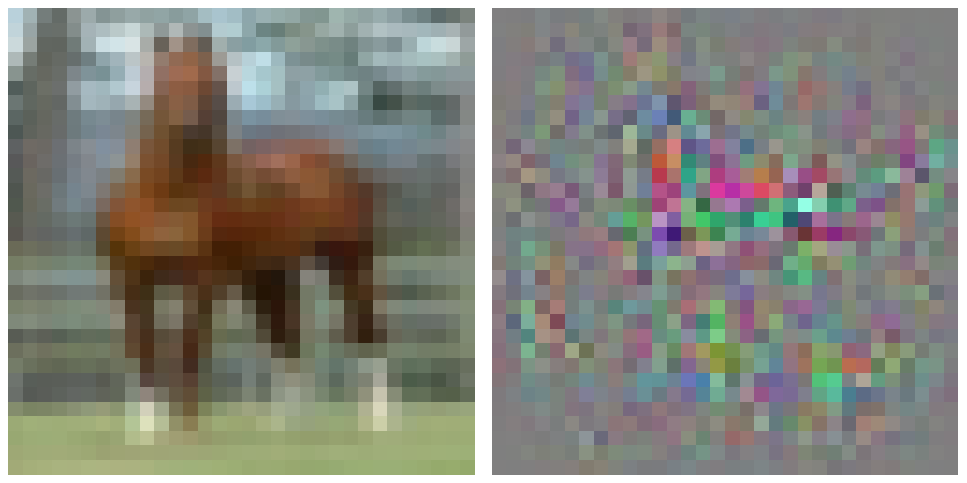
\includegraphics[height=2cm]{cifar10_carlini_wagner_caps.pdf} & 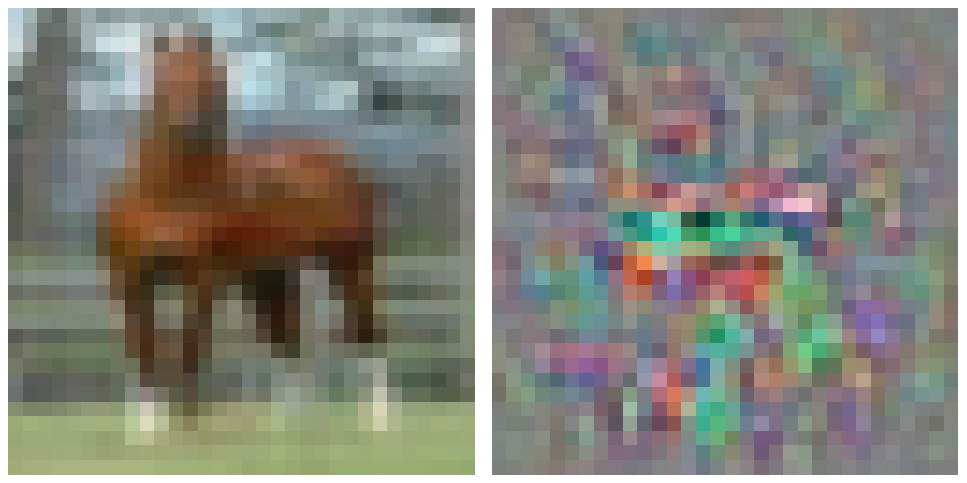
\includegraphics[height=2cm]{cifar10_carlini_wagner_conv.pdf}\\
	\\
	\raggedleft Boundary &
	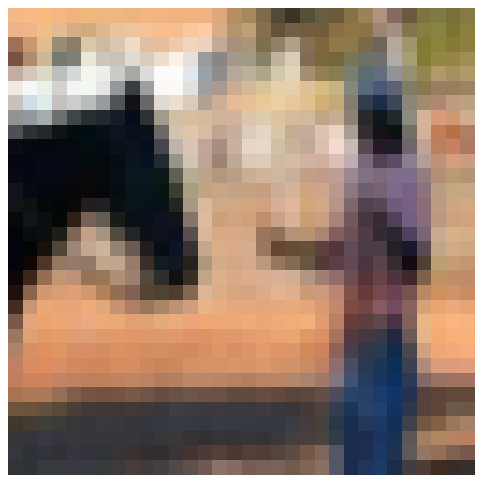
\includegraphics[height=2cm]{cifar10_boundary_attack_orig.pdf} & 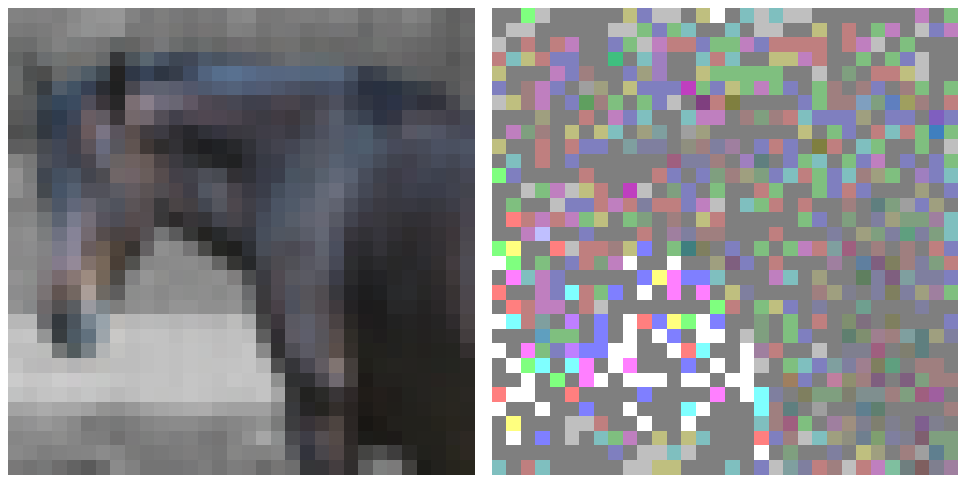
\includegraphics[height=2cm]{cifar10_boundary_attack_caps.pdf} & 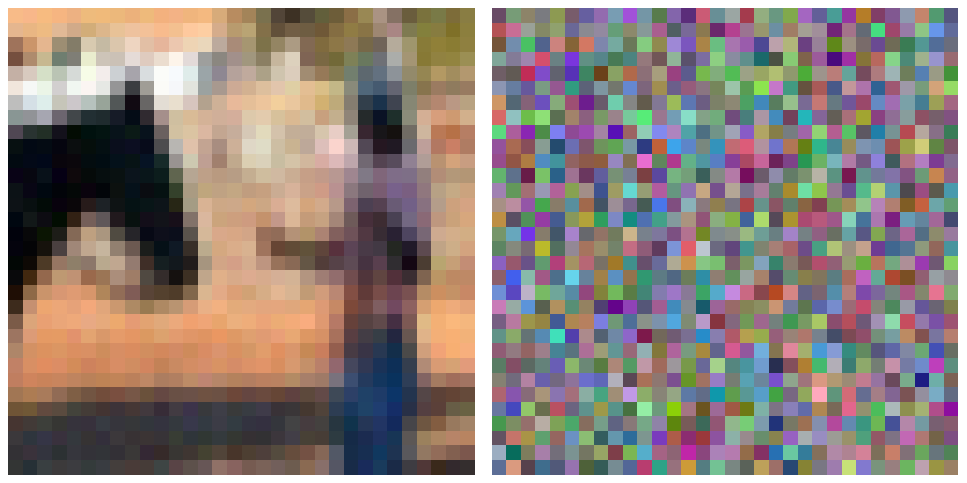
\includegraphics[height=2cm]{cifar10_boundary_attack_conv.pdf}\\
	\\
	\raggedleft DeepFool&
	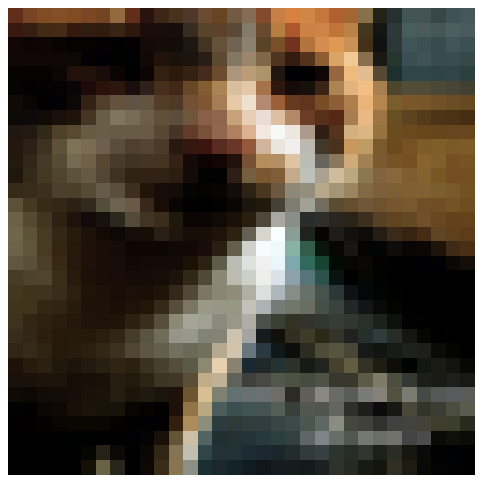
\includegraphics[height=2cm]{cifar10_deepfool_orig.pdf} & 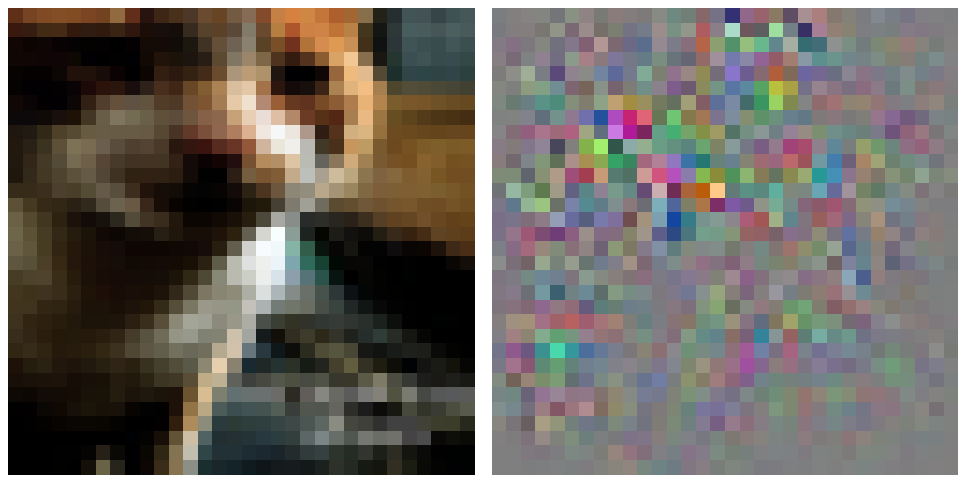
\includegraphics[height=2cm]{cifar10_deepfool_caps.pdf} & 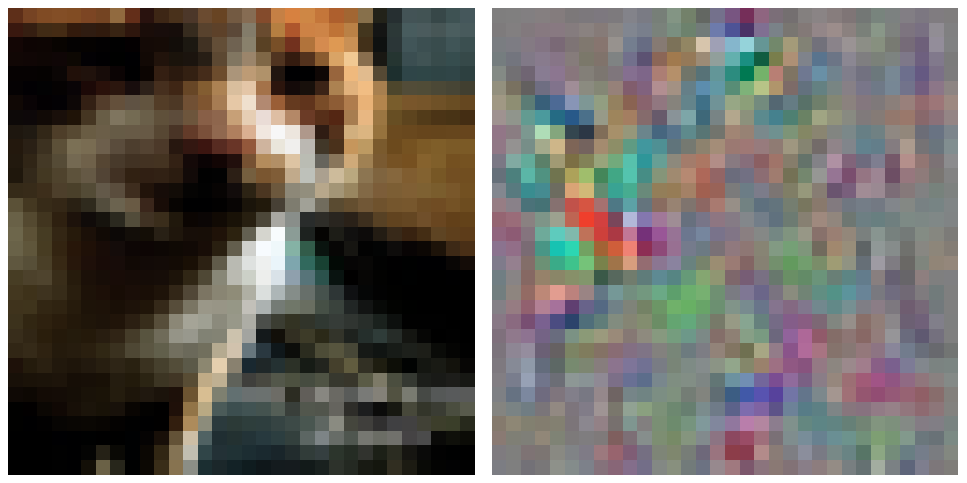
\includegraphics[height=2cm]{cifar10_deepfool_conv.pdf}\\
	\\
	\raggedleft Universal&
	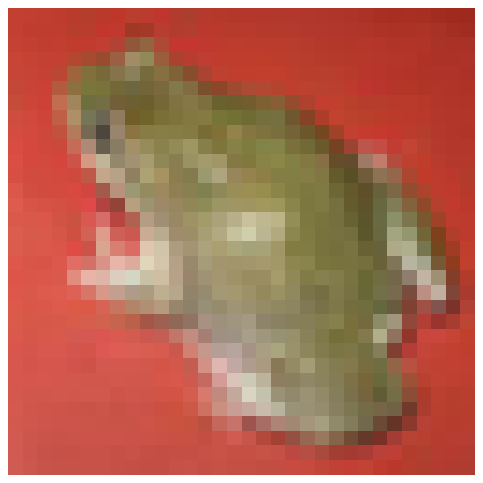
\includegraphics[height=2cm]{cifar10_universal_perturbation_orig.pdf} & 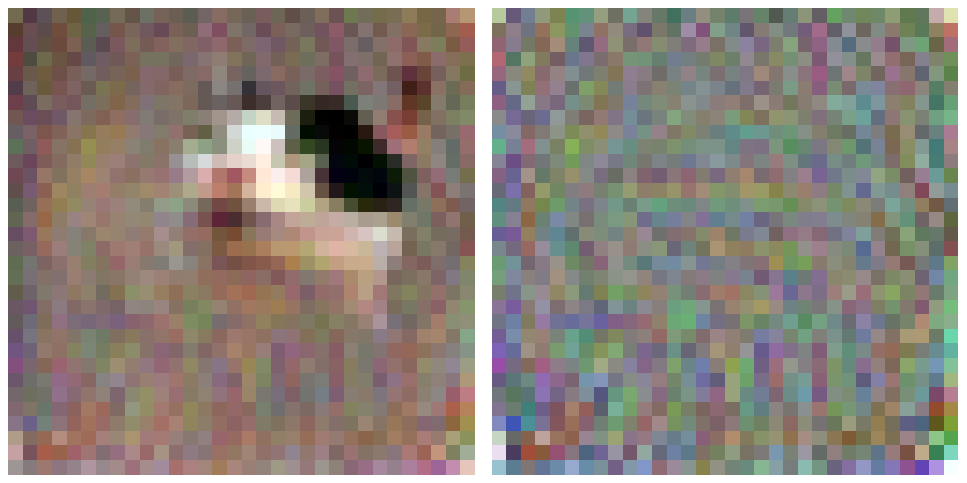
\includegraphics[height=2cm]{cifar10_universal_perturbation_caps.pdf} & 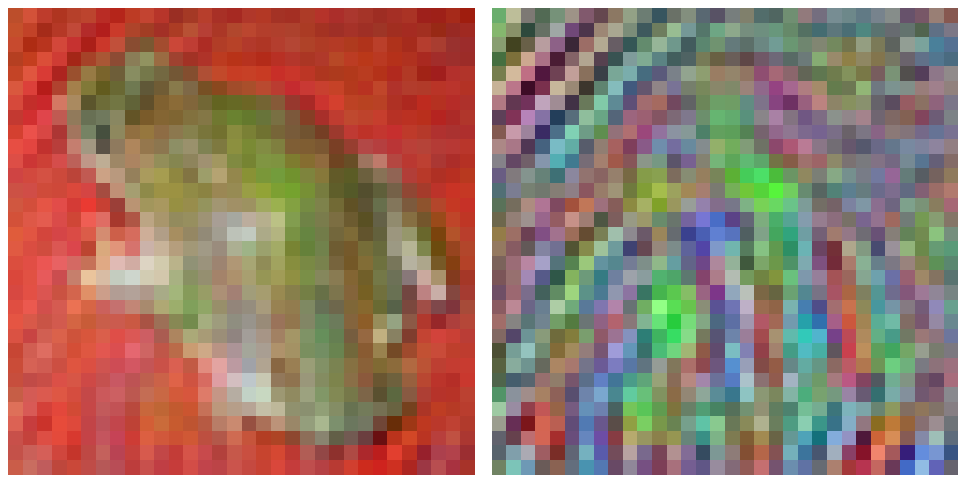
\includegraphics[height=2cm]{cifar10_universal_perturbation_conv.pdf}
\end{longtable*}
% This should count as a figure and not as a table
%\addtocounter{table}{-1}
\captionof{figure}[Adversarial examples on CIFAR-10]{Original images from the CIFAR-10 dataset (left), adversarial examples and perturbations for CapsNet (middle) and adversarial examples and perturbations for ConvNet (right). Pixel values of perturbation images are scaled for visibility.}
\label{fig:images}
\end{center}

\subsection{Robustness to Adversarial Attacks}

The most important aspect with respect to the dangers of adversarial attacks is how much an image has to be modified for an successful attack, i.e.\ the distance to the original image in some metric.
In our case this is the Euclidean norm, see \Cref{sec:attacks}.
These results are displayed in \Cref{tab:norms}.
On all datasets except MNIST the CapsNets is more susceptible to the Carlini-Wagner attack than the ConvNets.

\begin{table}
	\centering\
	\begin{tabular}{llcccc}
		\toprule
		Attack & Network       & MNIST & Fashion & SVHN & CIFAR-10  \\
		\midrule
		\multirow{2}{*}{CW} & ConvNet & {$1.40$} & $0.51$ & $0.67$ & $0.37$ \\
		& CapsNet            & $1.82$ & {$0.50$} & {$0.60$} & {$0.23$} \\
		\midrule
		\multirow{2}{*}{Boundary} & ConvNet & {$3.07$} & $1.24$ & $2.42$ & $1.38$ \\
		& CapsNet            & $3.26$ & {$0.93$} & {$1.88$} & {$0.72$} \\
		\midrule
		\multirow{2}{*}{DeepFool} & ConvNet & {$1.07$} & {$0.31$} & {$0.41$} & $0.23$ \\
		& CapsNet           & $2.02$ & $0.55$ & $0.80$ & {$0.16$} \\
		\midrule
		\multirow{2}{*}{Universal} & ConvNet & {$6.71$} & {$2.61$} & {$2.46$} & {$2.45$} \\
		& CapsNet           & $11.45$ & $5.31$ & $8.59$ & $2.70$ \\
		\bottomrule\\
	\end{tabular}
	\caption[Average perturbation norms]{Average perturbation norms for each attack and architecture}
	\label{tab:norms}
\end{table}

We observe the same trend for the adversarial examples calculated using the Boundary attack.
This means that CapsNets are in general neither more robust against white-box attacks nor against black-box attacks than ConvNets, as long as the attacks are sufficiently strong.
Against DeepFool however the CapsNets perform slightly better and have significantly higher adversarial perturbation norms for all datasets except CIFAR-10.

The biggest difference between the architectures is the behavior against universal perturbations, where the norms of the perturbations for the CapsNets are considerably higher for the MNIST, Fashion-MNIST and SVHN datasets. Especially the perturbations on SVHN calculated for the CapsNet are not just clearly visible, the original image is in some cases not recognizable anymore (see \Cref{fig:universal-img}).
Only the universal perturbations on CIFAR-10 have similar norms for the CapsNet and the ConvNet.

However, we have to mention that while the existence of adversarial perturbations with small norms shows the lack of robustness, proving resistance to adversarial attacks is vastly more difficult.
After all, adversarial perturbations with large norms can just be the result of an inadequate attack.

\citet{transfer} demonstrated the existence of \emph{cross-technique transferability} for a wide variety of machine learning techniques.
This means that adversarial examples constructed for a specific classifier may also be able to fool another classifier using a vastly different machine learning model.
Such transfer attacks can be seen as black-box attacks where the first model functions as a oracle (or substitute) for the second one.

\definecolor{dblue}  {RGB}{20,66,129}
\definecolor{norange}{RGB}{230,120,20}

\begin{wrapfigure}{O}{6.4cm}
	\centering
	%\scalebox{1}{%
		\begin{tikzpicture}
		\tikzset{
			node distance = 9em and 4em,
			sloped,
			box/.style = {%
				shape=rectangle,
				rounded corners,
				draw=dblue!70,
				fill=dblue!10,
				align=center,
				font=\fontsize{12}{12}\selectfont},
			arrow/.style = {%
				draw=dblue!70,
				line width=1mm,% <-- select desired width
				-{Triangle[length=3mm]},
				shorten >=1mm, shorten <=1mm,
				font=\fontsize{8}{8}\selectfont},
		}
		
		\node[box] at (0,0)(capsnet){CapsNet};
		\node[box] at (0,6)(convnet){ConvNet};
		\node[box] at (2,3)(pertconv){Perturbations};
		\node[box] at (-2,3)(pertcaps){Perturbations};
		\draw[arrow](capsnet) to [bend right,looseness=1] node[below] {calculate} (pertconv);
		\draw[arrow](convnet) to [bend right,looseness=1] node[above] {calculate} (pertcaps);
		\tikzset{
			node distance = 9em and 4em,
			sloped,
			arrow/.style = {%
				draw=norange!70,
				line width=1mm,% <-- select desired width
				-{Triangle[length=3mm]},
				shorten >=1mm, shorten <=1mm,
				font=\fontsize{8}{8}\selectfont},
		}
		
		\draw[arrow](pertcaps) to [bend right,looseness=1] node[below] {evaluate} (capsnet);
		\draw[arrow](pertconv) to [bend right,looseness=1] node[above] {evaluate} (convnet);
		
		\tikzset{
			node distance = 9em and 4em,
			sloped,
			arrow/.style = {%
				draw=norange!30,
				line width=1mm,% <-- select desired width
				-{Triangle[length=3mm]},
				shorten >=1mm, shorten <=1mm,
				font=\fontsize{8}{8}\selectfont},
		}
		\draw[arrow](pertcaps) to [bend right,looseness=1.2] node[above] {evaluate} (convnet);
		\draw[arrow](pertconv) to [bend right,looseness=1.2] node[below] {evaluate} (capsnet);
		\end{tikzpicture}%}
	\caption[Evaluation procedure]{Our evaluation procedure. The light orange arrows show the usual application of adversarial perturbations used in \Cref{tab:norms} while the dark orange arrows show the application used in \Cref{tab:transfer}.}
	\label{fig:eval}
\end{wrapfigure}

To measure the transferability we evaluate the fooling rate of the adversarial examples calculated for CapsNets when applied to the ConvNets and vice versa (see \Cref{fig:eval}). We define an image to \emph{fool} a network in the case of the untargeted attacks (Boundary, DeepFool, universal) if it is misclassified and in the case of targeted attacks (Carlini-Wagner) if it is classified as the target label for that the adversarial example was computed.

The transfer fooling rates (\Cref{tab:transfer}) for the Carlini-Wagner attack are quite small, even though we used a non-zero confidence parameter of $\kappa=1$.
The untargeted boundary and DeepFool attacks have higher fooling rates in general and match the result of \Cref{tab:norms} for most data sets, as in adversarial examples with high norms lead to a higher transfer fooling rate.
This is not the case for the Boundary attack with MNIST and the DeepFool attack with Fashion-MNIST. However the difference in fooling rates for the latter case is quite small and it is not surprising that MNIST would produce an outlier, since the adversarial perturbations for this data set are so large.

\begin{table}
	\centering
	\begin{tabular}{llcccc}
		\toprule
		Attack & Network       & MNIST & Fashion & SVHN & CIFAR-10  \\
		\midrule
		\multirow{2}{*}{CW} & ConvNet & $0.8\%$ & $1.2\%$ & $2.8\%$ & $2.4\%$ \\
		& CapsNet            & $2.0\%$ & $2.0\%$ & $3.8\%$ & $2.0\%$ \\
		\midrule
		\multirow{2}{*}{Boundary} & ConvNet & $8.8\%$ & $9.5\%$ & $10.5\%$ & $13.4\%$ \\
		& CapsNet            & $14.2\%$ & $14.6\%$ & $12.9\%$ & $26.1\%$ \\
		\midrule
		\multirow{2}{*}{DeepFool} & ConvNet & $4.3\%$ & $8.5\%$ & $13.5\%$ & $11.8\%$ \\
		& CapsNet           & $0.9\%$ & $10.9\%$ & $10.8\%$ & $14.1\%$ \\
		\midrule
		\multirow{2}{*}{Universal} & ConvNet & $4.9\%$ & $20.4\%$ & $35.0\%$ & $25.9\%$ \\
		& CapsNet           & $38.2\%$ & $25.7\%$ & $53.4\%$ & $47.2\%$ \\
		\bottomrule\\
	\end{tabular}
	\caption[Transfer fooling rates]{Fooling rates of adversarial examples calculated for a CapsNet and evaluated on a ConvNet and vice versa. For the universal attack we report the accuracy on the whole test set.}
	\label{tab:transfer}
\end{table}

The most noteworthy finding here are the fooling rates for the universal perturbations.
Although the norms of the CapsNet universal perturbations were much larger (see \Cref{tab:norms}), they perform poorly on the ConvNet, while the small perturbations computed for the ConvNet achieve relatively high fooling rates on the CapsNet.
Especially for SVHN the universal perturbations of the ConvNet are much more effective on the CapsNet than the perturbations computed on the CapsNet itself.

\subsection{Structural Analysis of Adversarial Examples}

While we have found, that CapsNets are not necessarily more robust against adversarial attacks, the low success rate of the transfer attacks and the radically different construction of the networks themselves suggest that there may be some structural difference between adversarial examples computed for ConvNets and those computed for CapsNets.

\subsubsection{Universal Attack t-SNE}

We use t-SNE \citep{tsne} to visualize the normalized universal perturbations created for the CapsNet and the ConvNet (see \Cref{fig:tsne}).
We discover that for all datasets there is a clear distinction between the perturbations calculated for the different architectures.
Although t-SNE can often distinguish the perturbations of models that are trained slightly differently, this is not just an outcome of this phenomenon.
By including another ConvNet in the diagram we find the clusters of the ConvNets almost perfectly matching while the cluster for the CapsNet is still separated.
This means, that the universal perturbation of CapsNets and ConvNets are intrinsically different.

In \Cref{fig:tsne} we can furthermore see subclusters based on the dataset splits used to calculate the perturbations.
These distinctions are however less pronounced with the other datasets besides CIFAR-10.

\begin{figure}
	\centering
	\begin{subfigure}{.5\textwidth}
	\includegraphics[scale=.5]{tsne_cifar10.pdf}
	\caption{CIFAR-10}
	\end{subfigure}%
	\begin{subfigure}{.5\textwidth}
	\includegraphics[scale=.5]{tsne_svhn.pdf}
	\caption{SVHN}
	\end{subfigure}
	\caption[t-SNE Plot of universal perturbations]{Two dimensional embedding of the universal perturbations calculated using t-SNE \citep{tsne}. The upper left cluster represents perturbations computed on a ConvNet, whereas the cluster in the lower right represents those calculated on a CapsNet. Perturbations with the same color were created using the same subset of test data.}
	\label{fig:tsne}
\end{figure}


\subsubsection{Singular Values of Adversarial Perturbations}
\citet{universal} considered singular values of the matrix containing normalized adversarial examples to determine, if adversarial examples lie in a low dimensional subspace. \\
For this purpose, let us denote with $\delta(x)$ the minimal adversarial perturbation for the input $x \in [0,1]^n$,
and $ N = \begin{bmatrix}
\frac{\delta(x_1)} {\norm{\delta(x_1)}},  ...,  \frac{\delta(x_k)} {\norm{\delta(x_k)}} 
\end{bmatrix}
\in \mathbb{R}^{n \times k}
$ for some $x_1, ..., x_k$ in the test set with $k > n$. \\
The perturbation vector $\delta(x)$ is orthogonal to the decision boundary, assuming it is reasonably smooth, therefore the singular values of $N$ give us information about the decision boundary. For example, for an binary linear classifier, $N$ would have a rank of one, i.e.\ only one non-zero singular value.

Accurately computing $\delta(x)$ is very challenging, so we use the result of the DeepFool attack as an approximation.
We computed $6000$ adversarial examples and plot the size of the singular values of the resulting Matrix $N$ together with a matrix containing columns randomly sampled from the unit sphere $S^{n-1}$ in \Cref{fig:svd}.

For both the CapsNets and the ConvNets the singular values decay much more quickly than those of the random matrix, confirming the findings of \citet{universal}.
In this regard the difference between CapsNets and ConvNets is inconclusive.
Whilst the curve of the CapsNet decreases more slowly than that of the ConvNet in the case of the CIFAR-10 dataset, the opposite occurs for the other cases.

\citet{fgsm} argue that the linear nature of neural networks is the cause for both their ability to generalize and their vulnerability to adversarial examples.
Indeed, many ConvNets model piecewise linear functions: max pooling and the ReLU activation are piecewise linear, while convolutional operations are linear, as are batch normalization and dropout at test time.
Due to the dynamic routing, CapsNets are generally not piecewise linear.
The linearity of the adversarial perturbations implied by their fast decaying singular values is however evidence that CapsNets also exhibit linear behavior similarly to ConvNets.

\begin{figure}
	\centering
	\begin{subfigure}{.5\textwidth}
		\includegraphics[scale=.5]{svd_cifar10.pdf}
		\caption{CIFAR-10}
	\end{subfigure}%
	\begin{subfigure}{.5\textwidth}
		\includegraphics[scale=.5]{svd_mnist.pdf}
		\caption{MNIST}
	\end{subfigure}
	
	\caption[Singular values of adversarial perturbations]{Singular values of the matrix containing normal vectors to the decision boundary}
	\label{fig:svd}
\end{figure}

\subsection{Effects on Activations}

To further the efforts in creating architectures robust to adversarial attack, we need to inspect which parts of the networks are responsible for their failure.
This is particularly important for the difference between CapsNets and ConvNets.
The primary capsule layer seems to need sufficiently complex features as input in order for the network to achieve adequate test performance.
For this reason, CapsNets usually start with a series of convolutional layers.
If an attack can perturb the leading convolutional layers in a considerable way, the following capsule layers will not be able to rectify the error.

To test this, we examine the difference of the layer's activations in out network when applied to unaltered and adversarial images. As a dimension and scale invariant metric we define
\begin{equation}
	d(z, w) = \frac{\norm[\infty]{z - w}}{\enspace \norm[\infty]{z}}
	\qquad \text{for original activation $z$ and perturbed activation $w$ .}
\end{equation}
This is related to the layer's Lipschitz constant.
Let $\phi$ be then function modeled by some layer and $z$ and $w$ the original and perturbed activation of the previous layer, then we have a lower bound for the Lipschitz constant with respect to the $L_{\infty}$-norm $K$ of the layer
\begin{equation}
K \geq \frac{d(\phi(z), \phi(w))}{d(z, w)} \cdot \frac{\norm[\infty]{\phi(z)}}{\norm[\infty]{z}}
\end{equation}
Low Lipschitz constants for every layer imply robustness to $L_p$ based attacks (in case $p \geq 1$).
Upper bounds for Lipschitz constants of convolutional and other common layers are known \citep{intriguing},
but have yet to be found for the routing-by-agreement algorithm.

Regarding CapsNets, we can differentiate between the activation of the instantiation parameters and that of the probabilities of presence.
Since we are using vector capsules, in our case the instantiation parameters is simply the complete output of a capsule layer and the probability of presence is given by the Euclidean norm of the capsules.

We compute the average activation error $d(z, w)$ for select layers over $128$ adversarial examples for our CIFAR-10 networks. Our CapsNet trained on CIFAR-10 begins with eight denseley connected convolutional layers and is therefore an apt choice for this comparison.
The results appear in \Cref{fig:activation}.

\begin{figure}
	\centering
	
	\begin{subfigure}{.5\textwidth}
		\includegraphics[scale=.5]{activation_error_conv.pdf}
		\caption{ConvNet}
	\end{subfigure}%
	\begin{subfigure}{.5\textwidth}
		\includegraphics[scale=.5]{activation_error_caps.pdf}
		\caption{CapsNet. Dashed lines are capsule norms.}
	\end{subfigure}
	\caption[Activation errors]{Activation errors of select layers. For the CapsNet we show the difference in the whole activation of each layer (instantiation parameters) and the difference of the capsule norms (probability of entity's presence).}
	\label{fig:activation}
\end{figure}

For the ConvNet the activation errors of the DeepFool, Boundary and Carlini-Wagner attacks are almost monotonically increasing.
This means, that not just a single layer is culpable for their deficiency to inhibit adversarial attacks, but instead the error accumulates over all the layers.
Curiously, the universal perturbations create substantially higher errors in the internal layers, but not so much in the final layer.
This is most likely the case, because a universal adversarial example not only has to disturb the activations of few features that are used for a specific image, but of all possible features. 
We want to mention that a high activation error in the last layer not necessarily corresponds to misclassifications of high confidence.
It can merely signify a change in \emph{many} class scores, not just those of the true class and the actually assigned false class.

The activation errors of the instantiation parameters match those of the ConvNet, meaning that even after convolutional layers in the beginning the error accumulates further.
While the error for the convolutional layers at the start seems large, we want to point out that the first error depicted is the result of eight convolutional layers and that the primary capsule layer has a direct skip connection to the input, but the activation error rises considerably in just the last two capsule layers.
We can notice that the error in the capsule norms starts with a dip in the primary capsule layer.
This is not automatically meaningful, since the two types of activations measure different aspects.
However, in all cases the error of the capsule norms escalates remarkably in the next capsule layer.
Together those results show not only the vulnerability of capsule layers themselves in general but also specifically that adversarial attacks are not treated as a capsule activation invariance by the routing-by-agreement algorithm.
